\documentclass[11pt,a4paper]{article}

% Core packages
\usepackage[utf8]{inputenc}
\usepackage[T1]{fontenc}
\usepackage{lmodern}
\usepackage{microtype}
\usepackage[margin=1in]{geometry}

% Bibliography
\usepackage[numbers,sort&compress]{natbib}

% Figures and tables
\usepackage{graphicx}
\graphicspath{{figures/}}
\usepackage{booktabs}
\usepackage{longtable}
\usepackage{array}
\usepackage{multirow}

% TikZ
\usepackage{tikz}
\usepackage{pgfplots}
\pgfplotsset{compat=1.18}
\usetikzlibrary{arrows.meta,positioning,shapes.geometric,fit,backgrounds,calc}

% Math
\usepackage{amsmath,amssymb,amsthm}

% Links
\usepackage[colorlinks=true,linkcolor=blue,citecolor=blue,urlcolor=blue]{hyperref}

% Headers
\usepackage{fancyhdr}
\pagestyle{fancy}
\fancyhf{}
\rhead{\thepage}
\setlength{\headheight}{14pt}

%% -----------------------------------------------------------------------
%% PAPER METADATA
%% -----------------------------------------------------------------------
\title{What Are We Not Testing? Region Coverage of Conversation Trajectories\\ from Agent Observability Traces}

% Author block (manual; no authblk dependency)
\author{Daniel Garc\'ia Pe\~na\\
  \small Department of Energy and Process Control, University of Oviedo, Oviedo, Spain\\
  \small AI Engineering, Unicaja Bank, Spain\\
  \texttt{info@iamdgarcia.com}}

\date{\today}

%% Theorem environments (mirror the companion papers)
\newtheorem{definition}{Definition}
\newtheorem{theorem}{Theorem}
\newtheorem{lemma}[theorem]{Lemma}
\newtheorem{proposition}[theorem]{Proposition}
\theoremstyle{definition}
\newtheorem{example}{Example}
\newtheorem{remark}{Remark}

\begin{document}

\maketitle

\begin{abstract}
Production conversational agents emit traces in standardized observability formats, and
LLM-based user simulators have become the standard tool for evaluating agents outside
production.
Yet these two artifacts have never been joined.
No published method maps observability traces to a discrete conversation state space with
terminal outcome classes, and no work quantifies which regions of conversational behavior a
simulator, or a candidate agent version, fails to cover.
We close this gap in two steps.
First, a formal extraction mapping $\tau$ converts standard agent-observability exports
(OpenTelemetry GenAI semantic conventions, OpenInference, LangSmith) into grammar walks over
the trajectory grammar $G=(Q,\Sigma,\delta)$, with terminal outcome classes and a cycle-depth
drift statistic.
Second, a region-coverage evaluation projects real and simulated walk collections into a
deterministic 2-D behavior plane anchored on production data, estimates where real
conversations live with a density grid under a shared relative occupancy threshold, and
reports coverage overall and per outcome class, together with the top-$K$ uncovered regions
and their nearest real exemplars: the tests you are not running, made concrete.
We also quantify the metric's own failure mode: at wide kernel bandwidths the density blur masks interior holes, so a kernel-free instance-coverage companion and a bandwidth ladder separate blur-limited from genuinely covered regimes.
The result is the trajectory atlas, a visualization and metric layer for sim-versus-real
transfer at the trajectory level.
A worked example on shipped fixtures (2 real / 1 simulated fixture conversations, 3 dialects;
an illustrative smoke test of runnability, not a population statistic) executes the full pipeline:
a 1-conversation simulated set covers 40.2\% of the occupied real regions (contained 45.3\%,
handoff 35.2\%), and the top uncovered regions name their nearest real exemplars. The extraction itself transfers: it runs verbatim, with no table tuning, on three third-party corpora (1{,}000 MultiWOZ 2.2 test dialogues, 4{,}201 Schema-Guided Dialogue test dialogues across 20 services, and 1{,}980 official tau-bench episodes of two production-grade LLM agents), whose own labels induce per-domain outcome distributions; the latter two carry native outcome truth (service-call results; environment-verified reward), which separates conversational closure from delivered outcome: untuned exact agreement is 55.3\% on Schema-Guided Dialogue (83.2\% with a close vocabulary calibrated on its dev split) --- an accuracy that is base-rate degenerate, since 99.8\% of test dialogues carry an effective call and a constant predictor scores 99.79\%, which is why the corpus's contribution is the verdict-vs-truth distance, not classifier score; a vocabulary-free semantic closing detector seeded from the dev split recovers 99.2\% of delivered closures (heuristic: 83.3\%) and transfers zero-shot in both directions; on real agent runs a conversational close is not evidence of success (45.8\% of contained-shape episodes failed the task, against 39.0\% of close-less ones), the confident-closing failure mode is common (21.7\% of failures end in a polite close with success claimed), and the walk's tool-retry depth acts as a transcript-only early warning that raises failure risk by $1.5\times$ on held-out episodes (two failed calls: 61.2\% fail rate vs 40.6\%, $p=4\times10^{-5}$); 31.7\% of real runs re-enter settled tool states, a loop human wizard corpora never exercise.
The extraction and coverage implementation ships as an open-source artifact with all checks
passing.
Third, a training-free trajectory-dynamics layer embeds each sampled window as a hybrid
semantic-plus-role-bound state, aligns it with a per-conversation counterfactual goal, and
exposes the confident-closing mode geometrically: on a 50-conversation pilot, abandoned
Schema-Guided Dialogue conversations end more goal-aligned than contained ones ($+0.73$ vs
$+0.48$), and four property tests measure why single-vector encodings cannot carry order
(order-change moves them $4$--$6\times$ less than content change) while a role-bound
sequential block recovers it.
\end{abstract}

\section{Introduction}
\label{sec:introduction}
% §1 Introduction
Evaluating a conversational agent outside production means talking to it with a simulator.
LLM-based user simulators now drive agent evaluation across task-oriented dialogue, tool use,
and agentic benchmarks \citep{sim2realAgentic2026,realUserSim2026,sierra2024taubench}.
The evaluation question every team asks is no longer ``did the agent pass'' but
``what kinds of conversations did we never even run'' ---
and no published method answers it measurably.

The raw material for an answer already exists on every deployment.
Production agents emit traces in standardized observability formats: the OpenTelemetry GenAI
semantic conventions (still marked Development as of October 2026 \citep{otelgenai2026}), the
OpenInference attribute specification \citep{openinference2026}, and LangSmith run trees
\citep{langsmith2026}.
Tooling mines these traces for failure prediction and benchmark construction
\citep{automataTraces2026,tracedance2026}, visualizes them as design-time graphs
\citep{graphoftrace2026}, and projects chat corpora into corpus-level maps
\citep{wildvis2024}.
But the conventions deliberately stop at the operation level: \texttt{gen\_ai.conversation.id}
is a linking key, not a conversation object.
The conversation-scale semantics --- which states the dialogue moved through, how it ended,
how deeply it regressed --- are left undefined by everyone.

Simulator validation, meanwhile, is measured at the wrong altitude for this question.
The 2026 sim2real wave compares response distributions in text space:
the distributional gap of \citet{distributionalGap2026} is response-level and text-only;
\citet{cds2026} scores distributional agreement of conversation-level statistics;
\citet{cue2026} calibrates user-simulator embeddings;
\citet{mirrorbench2026} benchmarks human-likeness of user proxies.
All of these ask ``do simulated responses look like real ones''.
None asks the structural question a test suite needs: \emph{which regions of conversational
behavior does the simulator exercise, and which real regions does it never touch?}
A simulator can match response distributions while never once producing the
clarify-then-abandon structure that a production cohort exhibits on bad-network days.

This paper joins the two artifacts.
We define a formal extraction mapping $\tau$ from standard observability exports to grammar
walks over the trajectory grammar $G=(Q,\Sigma,\delta)$ of our companion work
\citep{garcia2026grammar}, with terminal outcome classes and cycle depth as drift statistic.
We then define \emph{region coverage}: project real and simulated walk collections into a
2-D behavior plane whose basis is fit on the real set only, estimate where real conversations
live with a deterministic density grid, and measure which occupied regions the simulated set
reaches --- overall and per outcome class --- while the top-$K$ uncovered regions return their
nearest real exemplars: \emph{the tests you are not running}, made concrete and actionable.
The two clouds in one plane constitute the \emph{trajectory atlas}, the visualization and
metric layer for sim-versus-real transfer at the trajectory level.

Our contributions are:
\begin{enumerate}
  \item a formal extraction mapping $\tau$ from standard agent-observability formats
        (OTel GenAI, OpenInference, LangSmith) to trajectory-grammar walks with terminal
        outcome classes and cycle depth, shipped as a rule-based baseline whose classifier
        configuration is fully exposed, with an emission-model assumption stated so any
        calibrated state estimator can replace it without changing the interface
        (Section~\ref{sec:extraction});
  \item region-coverage evaluation: deterministic 2-D projection anchored on production,
        density-occupied real regions under a shared relative threshold, coverage
        overall and per outcome class, and top-$K$ uncovered regions with nearest real
        exemplars (Section~\ref{sec:coverage});
  \item the trajectory atlas as the visualization and metric layer for sim-versus-real
        comparison at the trajectory level, with a worked example on shipped fixtures and an
        evaluation protocol --- sensitivity sweep, class-conditional coverage, and a baseline
        ladder --- for paper-grade results (Sections~\ref{sec:atlas}
        and~\ref{sec:evaluation}).
\end{enumerate}

The paper is organized as follows.
Section~\ref{sec:background} recaps the grammar formalism, the distributional evaluation
lineage, and the verified facts about observability formats.
Section~\ref{sec:extraction} defines $\tau$.
Section~\ref{sec:coverage} defines region coverage.
Section~\ref{sec:atlas} presents the atlas and the worked example.
Section~\ref{sec:evaluation} gives the evaluation protocol.
Sections~\ref{sec:open_problems}--\ref{sec:conclusion} discuss open problems, limitations,
and conclusions.


\section{Background}
\label{sec:background}
% §2 Background
\subsection{The trajectory grammar}
We build on the trajectory grammar of our companion paper \citep{garcia2026grammar}, which we
summarize only to fix notation.
A conversation trajectory is a walk $\sigma = q_0 \to q_1 \to \cdots \to \theta$ over a finite
state space $Q$ with transition relation $\delta$ and alphabet $\Sigma$ of typed transitions.
The progress states are the stages a service dialogue moves through
($q_{\mathrm{greet}}, q_{\mathrm{auth}}, q_{\mathrm{intent}}, q_{\mathrm{tool}},
q_{\mathrm{clarify}}, q_{\mathrm{confirm}}, q_{\mathrm{close}}$), and every run ends in one of
four terminal outcome classes: contained ($\theta_{\mathrm{cont}}$), abandoned
($\theta_{\mathrm{aban}}$), human handoff ($\theta_{\mathrm{hand}}$), and compliance-escape
($\theta_{\mathrm{esc}}$).
The \emph{cycle depth} $D(\sigma)$ counts regressions --- returns to a state previously
settled --- and serves as the grammar's drift statistic.
The grammar's guarantees (early outcome prediction and intervention on partial conversations)
attach to its stopping layer under calibrated emissions; how the present paper relates to
those guarantees is discussed in Section~\ref{sec:extraction}.
Compliance-escape is an audit overlay inherited verbatim from the companion grammar; we do not
re-derive it here \citep{garcia2026grammar}.
The grammar sits inside a sibling program that bounds the same agents' realtime behavior on
both sides --- the latency floor of the onset \citep{garcia2026latencyfloor} and the cessation
floor of stopping \citep{garcia2026cessationfloor} --- where this paper adds the evaluation
side: what the conversation content of a test collection actually spans.

\subsection{Distributional evaluation of conversation}
A parallel line of work scores how simulated conversation compares to real conversation.
The Conversational Distribution Score measures distributional agreement of
conversation-level statistics between two populations \citep{cds2026}.
TurnBench evaluates turn-taking dynamics across spoken-dialogue domains
\citep{turnbench2026}.
MirrorBench asks whether user-proxy agents are indistinguishable from humans
\citep{mirrorbench2026}.
These metrics compare populations when both exist; none of them identifies \emph{which}
behavioral regions a collection fails to reach, which is the question an evaluation owner
must answer before trusting the comparison.

\subsection{Sim2real gaps in agent evaluation}
The sim2real line measures how far a simulator drifts from production users.
\citet{sim2realAgentic2026} document the sim2real gap for user simulation in agentic tasks;
\citet{distributionalGap2026} measure and mitigate a response-level distributional gap in
text; \citet{realUserSim2026} describe the ``Formalism Ceiling'' of grounded user simulation;
\citet{cue2026} calibrate user embeddings so simulators track real user states.
\citet{simulatorCollapse2026} show that a single frozen simulator systematically fails to
generalize in multi-agent reinforcement learning --- population-level evidence that simulator
deficiency is structural, not incidental.
All of these operate at the response or style level; the trajectory level --- which
conversation structures a simulator exercises --- remains unmeasured.

\subsection{Trace mining and observability formats}
Trace mining recovers structure from execution logs: automata for failure and next-step
prediction \citep{automataTraces2026}, behavior benchmarks from deployment traces
\citep{tracedance2026}, workflow graphs for scientific agents \citep{graphoftrace2026},
and corpus-level visual maps of chat logs \citep{wildvis2024}.
Early outcome prediction from partial transcripts \citep{nourbakhsh2026tracer} and
trajectory-structure diagnostics for coding agents \citep{resolveRate2026} use traces as
evaluation signal; early-prediction evaluation trade-offs are measured by
\citet{earlyeval2026} and label-reliability over agent trajectories by
\citet{falsesuccess2026}; full-episode outcome comparison is the paradigm of
$\tau$-bench \citep{sierra2024taubench}; \citet{salesforce2025workflows} extract dialog
workflows from conversations.
Conformance contracts for agent frameworks --- machine-checked checkpoint/resume semantics
\citep{resume2026} and control-primitive enforcement gaps \citep{stopmeansstop2026} ---
establish that framework behavior can and should be checked against explicit contracts; the
present paper brings the same discipline to the extraction interface.

On the format side, three facts (verified against the published specifications and
repositories in October 2026) fix the extraction problem's boundary:
\begin{itemize}
  \item \textbf{OTel GenAI} semantic conventions live in their own repository
        \citep{otelgenai2026}, remain under Development status, define per-call spans
        (\texttt{invoke\_agent}, \texttt{execute\_tool}), and expose the conversation
        identifier \texttt{gen\_ai.conversation.id} only as a Conditionally Required linking
        key --- there is no conversation object, and message content lives in Opt-In
        client-inference attributes.
  \item \textbf{OpenInference} ships the most complete stable attribute specification
        (span kinds LLM/AGENT/TOOL/CHAIN under \texttt{openinference.span.kind}, structured
        inputs, outputs, and tool-call lists) on the same span envelope.
  \item \textbf{LangSmith} exports run trees whose \texttt{parent\_run\_id} grouping is the
        de-facto evaluation-side session artifact.
\end{itemize}
All three reduce to per-operation records with session identifiers; none assigns
conversation states, outcomes, or drift.
Voice-physics channels (barge-in, endpointing, tool latency) die at the transport boundary in
current stacks and are out of scope here, appearing only as an optional appendix extension of
the companion grammar \citep{garcia2026grammar}.

\subsection{Position against the nearest neighbors}
Table~\ref{tab:neighbors} makes the deltas explicit.
\begin{table}[t]
\centering
\small
\begin{tabular}{@{}p{2.9cm}p{2.6cm}p{3.1cm}p{3.6cm}@{}}
\toprule
 & \textbf{Axis} & \textbf{They provide} & \textbf{They leave unclaimed} \\
\midrule
\citet{distributionalGap2026} &
  response distributions &
  text-level real-vs-sim divergence &
  grammar walks, region coverage, outcome classes \\
\citet{automataTraces2026} &
  automata from traces &
  failure/next-step prediction &
  conversation semantics, outcome classes, atlas \\
\citet{graphoftrace2026} &
  workflow graphs &
  design-time execution graphs &
  outcome classes, population-level coverage \\
\citet{tracedance2026} &
  trace benchmarks &
  benchmark construction from traces &
  state space, sim-vs-real atlas \\
\citet{wildvis2024} &
  corpus visualization &
  million-scale chat-log UMAP &
  agent spans, grammar, per-class semantics \\
\citet{resolveRate2026} &
  process diagnostics &
  trajectory-structure statistics &
  observability ingestion, region coverage \\
\bottomrule
\end{tabular}
\caption{The nearest neighbors and the axis each leaves unclaimed.
The extraction mapping $\tau$ plus region coverage occupy the joint gap.}
\label{tab:neighbors}
\end{table}


\section{The Extraction Mapping $\tau$}
\label{sec:extraction}
% §3 The extraction mapping tau
The extraction mapping $\tau$ converts a standard observability export into a grammar walk.
This section defines its three stages --- normalization, state inference, walk construction ---
as shipped in the open-source implementation,\footnote{\url{https://github.com/iamdgarcia/trace2grammar}}
and states the assumption that governs what the paper's coverage results inherit.
Figure~\ref{fig:pipeline} shows the pipeline.

\begin{figure}[t]
\centering
\resizebox{\textwidth}{!}{% The extraction pipeline: three observability dialects in, coverage atlas out.
% Layout: positioning-relative (border distances), so boxes cannot overlap no matter
% how wide their labels set them. Bottom row is a boustrophedon snake (right to left),
% which removes the old long curved arrow from features back to PCA.
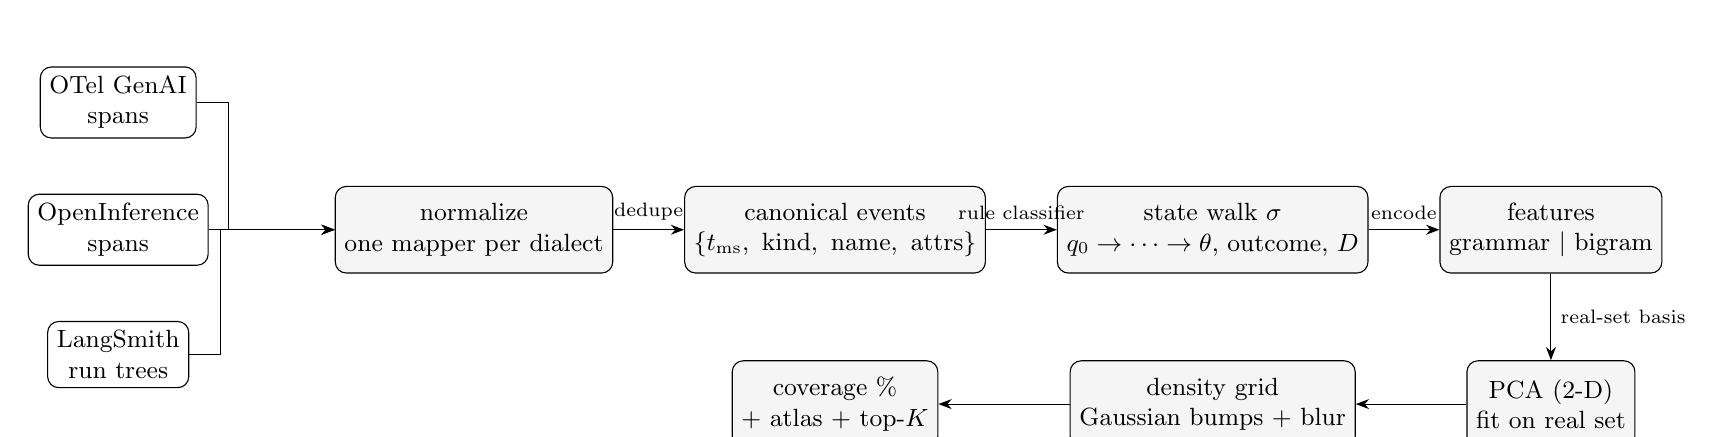
\begin{tikzpicture}[>=Stealth, font=\small,
  box/.style={draw, rounded corners, align=center, minimum height=8mm},
  stage/.style={draw, rounded corners, align=center, minimum height=11mm, fill=black!4},
  ev/.style={->,>=Stealth},
  node distance=7mm and 9mm]
  % dialects (left, stacked)
  \node[box] (otel) {OTel GenAI\\spans};
  \node[box, below=7mm of otel] (oinf) {OpenInference\\spans};
  \node[box, below=7mm of oinf] (lsm) {LangSmith\\run trees};
  % top row, chained by borders (middle dialect anchors the entry stage)
  \node[stage, right=16mm of oinf] (norm) {normalize\\one mapper per dialect};
  \node[stage, right=of norm] (evts) {canonical events\\$\{t_{\mathrm{ms}},\ \mathrm{kind},\ \mathrm{name},\ \mathrm{attrs}\}$};
  \node[stage, right=of evts] (walk) {state walk $\sigma$\\$q_0 \to \cdots \to \theta$, outcome, $D$};
  \node[stage, right=of walk] (feat) {features\\grammar $|$ bigram};
  % bottom row (snake, right to left)
  \node[stage, below=11mm of feat] (proj) {PCA (2-D)\\fit on real set};
  \node[stage, below=11mm of walk] (grid) {density grid\\Gaussian bumps + blur};
  \node[stage, below=11mm of evts] (cov) {coverage \%\\+ atlas + top-$K$};
  % arrows
  \draw[ev] (otel.east) -- ++(4mm,0) |- (norm.west);
  \draw[ev] (oinf.east) -- (norm.west);
  \draw[ev] (lsm.east) -- ++(4mm,0) |- (norm.west);
  \draw[ev] (norm) -- (evts) node[midway,above,font=\scriptsize]{dedupe};
  \draw[ev] (evts) -- (walk) node[midway,above,font=\scriptsize]{rule classifier};
  \draw[ev] (walk) -- (feat) node[midway,above,font=\scriptsize]{encode};
  \draw[ev] (feat) -- (proj) node[midway,right,font=\scriptsize]{real-set basis};
  \draw[ev] (proj) -- (grid);
  \draw[ev] (grid) -- (cov);
\end{tikzpicture}
}
\caption{The extraction-and-coverage pipeline.
Three observability dialects (OTel GenAI, OpenInference, LangSmith; $\tau$-bench episodes as a
fourth evaluation-side dialect) are normalized into a canonical event stream, classified into a
grammar walk with outcome class and cycle depth, encoded as feature vectors, projected onto a
2-D plane fit on the real set, and scored for region coverage.}
\label{fig:pipeline}
\end{figure}

\subsection{Canonical event stream}
Every dialect is reduced to one format-agnostic event stream
$e = (t_{\mathrm{ms}}, \mathrm{kind}, \mathrm{name}, \mathrm{attrs})$ with event kinds
\begin{equation}
\begin{aligned}
\mathrm{kind} \in \{\,&\texttt{user\_msg},\ \texttt{assistant\_msg},\ \texttt{tool\_call},\\
&\texttt{tool\_result},\ \texttt{tool\_error},\ \texttt{hangup},\\
&\texttt{handoff},\ \texttt{session\_end}\,\}.
\end{aligned}
\label{eq:kinds}
\end{equation}
One normalization function per dialect maps its export shape onto
Equation~\eqref{eq:kinds}:
\begin{itemize}
  \item \texttt{\_normalize\_otel} --- OTel GenAI spans, conversation-scoped, with the
        \texttt{gen\_ai.*} attributes of \texttt{invoke\_agent} and
        \texttt{execute\_tool} calls;
  \item \texttt{\_normalize\_openinference} --- typed OpenInference spans:
        \texttt{input.value}, \texttt{output.value};
  \item \texttt{\_normalize\_langsmith} --- runs grouped by \texttt{parent\_run\_id};
  \item \texttt{\_normalize\_taubench} --- transcript turns plus the environment-verified
        reward, which drives the terminal outcome (a documented public analogue for
        production containment).
\end{itemize}
Timestamps are normalized to milliseconds (epoch nanoseconds or ISO timestamps depending on
dialect), attributes are flattened, and adjacent duplicate events are deduplicated.
Everything downstream of the canonical stream is format-agnostic; adding a dialect is one
normalization function, which is what keeps $\tau$ maintainable as the specification landscape
shifts --- the OTel GenAI conventions are still under Development status
\citep{otelgenai2026}.

\subsection{State inference as a config-exposed classifier}
The second stage maps the canonical stream to a grammar walk
$\sigma = q_0 \to q_1 \to \cdots \to \theta$ with states
$Q = \{q_{\mathrm{greet}}, q_{\mathrm{auth}}, q_{\mathrm{intent}}, q_{\mathrm{tool}},$
$q_{\mathrm{clarify}}, q_{\mathrm{confirm}}, q_{\mathrm{close}}\}$ and terminals
$\Theta = \{\theta_{\mathrm{cont}}, \theta_{\mathrm{aban}}, \theta_{\mathrm{hand}},$
$\theta_{\mathrm{esc}}\}$ \citep{garcia2026grammar}.
The seven states are not a domain model: they are the domain-independent phases of a
tool-calling dialogue (opening, identity, intent, execution, repair, confirmation, closing).
The set is a superset --- a walk uses the sub-sequence the deployment exhibits, so an agent
without authentication simply never emits $q_{\mathrm{auth}}$ --- and what varies per vertical
is which surface forms trigger each transition, never the phases themselves.
The baseline classifier is deliberately rule-based: keyword and regex pattern tables
(authentication tool names, handoff tool names, user clarification and confirmation phrases,
assistant closing phrases, explicit terminal event names) plus sequencing rules (a user
clarification re-opens the current settled state and increments cycle depth; tool errors with
recovery stay in $q_{\mathrm{tool}}$; explicit hangup and handoff events drive the terminal).
Every pattern lives in an \texttt{ExtractionConfig} dataclass, so a domain owner adapts the
mapping to a new vertical (banking, retail, IT support) by editing configuration, not code.

This is a heuristic, and the paper's claim does not depend on it being more.
The contribution is the \emph{interface}: deterministic walks with typed transitions that any
downstream measurement can consume.
The learned emission mapper that will replace the pattern tables is future work
(Section~\ref{sec:open_problems}); the configuration tables double as its training-data
generator.

\begin{definition}[Extraction mapping]
\label{def:tau}
$\tau : \mathcal{D} \to \Sigma^* \times \Theta \times \mathbb{N}$ maps an observability export
$d \in \mathcal{D}$ to a walk $\sigma$ over states $q \in Q$ with typed transitions from
$\Sigma$, an outcome class $\theta \in \Theta$, and a cycle depth $D(\sigma)$, such that every
walk step is grounded in a canonical event of Equation~\eqref{eq:kinds} and every terminal
class is decided by an explicit rule over terminal events, tool-error counts, or (for
evaluation dialects) environment-verified outcomes.
\end{definition}

\subsection{Outcome classes and cycle depth}
The walk ends in exactly one terminal class.
Contained ($\theta_{\mathrm{cont}}$) requires an explicit close with no unresolved tool
errors; handoff ($\theta_{\mathrm{hand}}$) is forced by handoff-typed tools or events;
abandoned ($\theta_{\mathrm{aban}}$) is the absence of a terminal event at stream end;
compliance-escape ($\theta_{\mathrm{esc}}$) is the audit overlay inherited from the companion
grammar \citep{garcia2026grammar}, computed as a post-hoc check rather than a walk state.
Cycle depth $D(\sigma)$ counts regressions to settled states --- the drift statistic that
distinguishes a healthy clarify loop from an endless one.

\subsection{The emission-model assumption, stated honestly}
The guarantees of the companion grammar attach to its \emph{stopping} layer under calibrated
emissions \citep{garcia2026grammar}.
$\tau$ supplies deterministic emissions (pattern tables), so this paper's coverage results
inherit the walk \emph{semantics} only --- state identity, transition typing, outcome
decidability --- and none of the prediction guarantees.
This is the honest dependency direction: the coverage metric is defined on walks, its
correctness claim is invariant to how walks are produced, and a calibrated state estimator
can replace \texttt{infer\_states()} without changing any downstream definition.
What the baseline does add is reproducibility: the same export always yields the same walk,
which Section~\ref{sec:evaluation} exploits to make sensitivity sweeps exact.


\section{Region Coverage}
\label{sec:coverage}
% §4 Region coverage
Region coverage answers one question: given real conversation walks and a simulated (or
candidate-agent) set, \emph{which occupied regions of conversational-behavior space does the
simulated set reach, and which does it never touch?}
The pipeline is deterministic and standard-library-only: features, projection, density,
threshold, coverage.
Figure~\ref{fig:coverage} shows the geometry.

\begin{figure}[t]
\centering
\includegraphics[width=0.98\textwidth]{fig_coverage}
\caption{The coverage geometry, computed on the artifact's fixture set (2 real / 1 simulated
walks; deterministic pipeline, $\rho{=}24$, $\beta{=}0.12$, $\varepsilon{=}0.05$).
(a) The three fixture walks in the real-anchored 2-D behavior plane: at this scale the
real cloud spans three outcome regions and the single simulated walk lands inside one.
(b) The density grid over the real cloud; the 256 occupied cells are those with real density
$d$ above $\varepsilon \cdot \mathrm{core}$, where $\mathrm{core} = \max(\mathrm{p99},\ 0.5\cdot\mathrm{peak})$
of the smoothed real field, mirroring the threshold definition above.
(c) Occupied cells split into covered (103, sim point inside or sim kernel mass above
threshold) and uncovered (153); each uncovered cell carries its nearest real exemplar ---
the test you are not running.}
\label{fig:coverage}
\end{figure}

\subsection{Feature encodings}
Each walk $\sigma$ with outcome $\theta$ and cycle depth $D$ becomes a vector under one of two
encodings.
The \textbf{grammar encoding} is
\begin{equation}
\phi_{\mathrm{gram}}(\sigma) = \big[\,|\sigma|,\ \mathrm{dur}(\sigma),\ D,\ \mathrm{visits}(q)\ \forall q \in Q,\ \#\texttt{tool\_call},\ \#\texttt{tool\_error},\ \mathbb{1}[\theta]\,\big],
\label{eq:gram}
\end{equation}
a structural fingerprint: walk length, duration, cycle depth, per-state visit counts,
tool-call and tool-error counts, and a terminal one-hot.
The \textbf{bigram encoding} is the histogram of the first $k$ state-to-state transitions
($k=6$ in all experiments, fixed by construction and not swept), flattened in a fixed
alphabet order --- a local-order fingerprint that ignores global statistics.
Both are z-normalized per column with the statistics computed on the real set only
(consistent with the real-anchored projection below), plus a zero-variance guard (constant
columns map to zero, no NaN), so a collection with one terminal class still projects cleanly.
The encodings are deliberately shallow: they measure structure, not semantics.
A paraphrase pair whose conversations have identical structure lands on the same point ---
the honest cost of the deterministic baseline, revisited in
Section~\ref{sec:evaluation}.

\subsection{Projection anchored on the real set}
All vectors are projected to 2-D by principal component analysis computed with power iteration
and deflation, \textbf{fit on the real set only}.
The design commitment is that production defines the behavior space: the principal axes are
estimated from real walks, and simulated points are projected onto those same axes.
Fitting jointly would let the simulated set move the axes --- a simulator collapsing onto one
behavior mode would shrink the plane onto that mode and hide exactly the deficiency the metric
exists to expose.
The projection is also deterministic (no stochastic neighborhood embedding, contrast
\citep{wildvis2024}): the same collections always produce the same plane, the same grid, and
the same coverage number, which makes the protocol of Section~\ref{sec:evaluation} exact
rather than sampled.

\subsection{Density and the shared threshold}
Real density is estimated by Gaussian-bump accumulation on a $\rho \times \rho$ grid covering
the real extent (padded by 15\%), followed by box-blur smoothing with bandwidth
$\sigma = \beta \rho$ cells.
Occupancy uses a \emph{shared relative threshold}: with $p_{99}$ the 99th percentile and
$\mathrm{peak}$ the maximum of the blurred real field, a cell is occupied when its real
density exceeds
\begin{equation}
\varepsilon \cdot \mathrm{core}, \qquad \mathrm{core} = \max\!\big(p_{99},\ 0.5 \cdot \mathrm{peak}\big).
\label{eq:threshold}
\end{equation}
The simulated field is accumulated on the same grid \emph{normalized by the real field's
peak}, not by its own peak: self-normalization would rescale a deficient sim set to fill the
plane and destroy the relative magnitudes that coverage compares.
A single threshold then governs both clouds --- occupancy for real, coverage for sim --- which
is what makes the two percentages commensurable.

\paragraph{The kernel-masking failure mode.}
The bandwidth that makes the kernel estimate smooth enough to define occupancy is also what
hides interior holes: a sim point's Gaussian bump spreads over $\approx (2\sigma)^2$ cells,
so at the shipped $\beta = 0.12$ ($\sigma = 2.88$ cells on a $24 \times 24$ grid) a single
simulated region deposits above-threshold mass a quarter-grid away from itself.
On the artifact's production-shaped sample set (500 conversations), a deliberately deficient
simulator --- 28 conversations, \emph{all} contained, zero abandonment, zero handoff ---
scores $96.3\%$ region coverage with per-class numbers of $100\%$ abandonment and $99\%$
handoff: the blur fills the holes the metric exists to name, and uncovered cells survive
only at the low-density fringe or under catastrophic collapse.
The regime that discriminates simulators is $\beta \le 0.04$ ($\sigma \le 1$ cell): the same
deficient simulator drops to $65\%$ overall and $41\%$ handoff, while a diverse simulated
set holds $100\%$.
Two structural consequences follow, and both are protocol requirements
(Section~\ref{sec:evaluation}): the sensitivity sweep must extend its bandwidth ladder down
into the discriminating regime instead of stopping at $0.08$, and region coverage must ship
with an instance-level companion (Definition~\ref{def:instance}) whose verdict does not
depend on the blur.

\subsection{Coverage, per-class coverage, and edge handling}
\begin{definition}[Region coverage]
\label{def:coverage}
Let $O$ be the occupied cell set (Equation~\eqref{eq:threshold}).
A cell is \emph{covered} when a simulated point falls inside it or the smoothed simulated
kernel places at least $\varepsilon \cdot \mathrm{core}$ relative mass in it.
The coverage of a set $S$ is $c(S) = |C|/|O|$ with $C \subseteq O$ the covered cells;
the \emph{class-conditional} coverage $c_\theta(S)$ restricts $O$ to cells whose nearest real
exemplar has outcome class $\theta$.
\end{definition}
\begin{definition}[Instance coverage]
\label{def:instance}
With $r$ the median nearest-neighbor distance of the real set in the projection plane, the
instance coverage of a simulated set $S$ is
$i(S) = \frac{1}{|R|} |\{x \in R : \exists s \in S,\ \lVert x - s\rVert \le r\}|$.
It is the probability that a real conversation has a simulated neighbor at the scale at
which real conversations resemble each other; the kernel does not participate, so an
interior hole cannot be blurred away.
Its radius $r$ is not a free hyperparameter: it is read off the real collection itself,
which keeps the real-anchored discipline of the projection.
\end{definition}
Simulated points outside the grid are dropped, not clamped: a sim point ten extents away must
not masquerade as a corner point.
Per-class coverage is what stops a majority class from hiding a failure --- a simulator can
cover 90\% of contained regions while covering 0\% of abandonment regions, and only the
class-conditional number exposes it --- but Definition~\ref{def:coverage} computes classes
from nearest-exemplar labels, and the kernel that blurs mass across the plane blurs class
membership with it; $i_\theta(S)$, the instance coverage restricted to class-$\theta$ real
conversations, is the number that resists both failure modes.
Both conditionings ride the same definition at any label granularity. The outcome classes
$\Theta$ are the \emph{shape} taxonomy of the conversation (how it ended); an \emph{operativa}
label --- the business operation the call was about (appointment, dispute a charge, account
access, \ldots), read off the domain tool names and the opening user utterance in the trace
itself --- is the \emph{business} taxonomy (what it was for). The shape classifier deliberately
collapses all intents into $q_{\mathrm{intent}}$; collapsing is not erasing, because the
operativa stays a per-walk label, and the class-conditional and instance numbers above apply
verbatim with $\theta$ ranging over operativas instead of outcomes. A simulator can then fail
one operativa while passing another --- the per-operativa table, not the global number, is
the actionable report.

\subsection{The recommendation loop: top-$K$ uncovered regions}
Coverage percentages localize the deficit in aggregate; the actionable unit is the individual
uncovered region.
Uncovered cells are ranked by local real density, neighbors within a Chebyshev distance of 2
are deduplicated, and the top-$K$ survivors each report their nearest real exemplar ---
conversation, outcome class, cycle depth, duration, first user utterance.
Each exemplar is a scenario seed: hand it to the simulator as a conditioning target (the
log-conditional ladder of Section~\ref{sec:evaluation}), regenerate, and re-measure.
The loop --- uncovered region $\to$ nearest real exemplar $\to$ simulator scenario $\to$
coverage delta --- is the metric's reason to exist inside an evaluation pipeline rather than
as a dashboard.


\section{The Trajectory Atlas}
\label{sec:atlas}
% §5 The trajectory atlas
The trajectory atlas renders the coverage computation as one behavior plane: real walks as
blue dots, simulated walks as orange diamonds, uncovered cells shaded red with
nearest-exemplar tooltips, outcome classes readable by position (and by per-class views as
small multiples).
It is simultaneously the paper's worked example and the artifact's operational interface.
Figure~\ref{fig:atlas} shows the schema.

\begin{figure}[t]
\centering
\includegraphics[width=0.9\textwidth]{fig_atlas}
\caption{The trajectory atlas, rendered from the artifact's coverage computation (same
deterministic run as Figure~\ref{fig:coverage}: 2 real / 1 simulated fixture walks,
rank-deficient basis at $n{=}2$ --- a smoke test of runnability, §\ref{sec:evaluation}).
Red cells are the 153 occupied-but-uncovered regions (top-3 by local real density outlined);
each carries its nearest real exemplar.
A concentrated sim cloud with a small radius (over-cooperative collapse) and a scattered sim
cloud with uncovered lobes is the typical deficient configuration.}
\label{fig:atlas}
\end{figure}

\subsection{Reading the atlas}
Three configurations recur.
\emph{Collapse}: the sim cloud concentrates on one real lobe (the over-cooperative user who
never abandons, never escalates --- cf.\ the Formalism Ceiling \citep{realUserSim2026} and the
human-likeness failures of \citep{mirrorbench2026}); coverage is high on the majority class
and near zero elsewhere.
\emph{Scatter}: the sim cloud spreads where real conversations never go --- off-distribution
generation that inflates the plane without measuring anything; the shared threshold of
Equation~\eqref{eq:threshold} keeps these points from manufacturing coverage, and
out-of-grid points are dropped rather than clamped.
\emph{Coverage with holes}: the sim cloud overlaps real mass but misses specific occupied
cells --- the most actionable configuration, because the holes come with named exemplars.
Cross-model comparison is legitimate by design: real logs and simulated runs may come from
different vendors and model generations, and the representation comparison rests on
cross-model convergence of layer representations \citep{layersSimilarDepths2025} and the
trajectory-geometry vocabulary \citep{trajectoryGeometry2026}.

\subsection{Worked example on shipped fixtures}
The open-source artifact ships fixtures in three dialects and regenerates every number below
from a single command.
The worked example uses 3 conversations across 3 dialects --- two real (one OTel GenAI export,
one OpenInference export) and one simulated (a LangSmith export) --- under the grammar feature
encoding, a $24 \times 24$ grid, $\varepsilon = 0.05$, bandwidth $\beta = 0.12$.
The real set occupies 256 grid cells; the 1-conversation simulated set covers 103 of them.

\begin{quote}
\small
\texttt{coverage: 40.2\% overall | per class: contained 45.3\%, handoff 35.2\%}
\end{quote}

\begin{table}[t]
\centering
\small
\begin{tabular}{@{}clllc@{}}
\toprule
\textbf{Rank} & \textbf{Grid cell} & \textbf{Local density} & \textbf{Nearest real exemplar (first user utterance)} & \textbf{Class} \\
\midrule
1 & (2,\,11)  & 0.86 & ``No puedo entrar en mi banca online'' & handoff \\
2 & (21,\,12) & 0.86 & ``Hola, quiero consultar el saldo de mi cuenta'' & contained \\
3 & (2,\,14)  & 0.54 & ``No puedo entrar en mi banca online'' & handoff \\
\bottomrule
\end{tabular}
\caption{Top-3 uncovered regions from the worked example (as reported by the shipped CLI).
Each names its nearest real exemplar --- the tests the simulated set is not running.
Exemplars are shown in the fixture's original language (Spanish); the pipeline is
language-agnostic by construction, with clarification/confirmation pattern tables as the only
language-coupled component.}
\label{tab:topk}
\end{table}

The interpretation is the paper's pitch in one line: a one-conversation simulated set covers
under half of the conversational-behavior regions that the real set occupies --- and the
uncovered regions are not an abstraction, they are named conversations with outcome classes
and cycle depths (Table~\ref{tab:topk}).
The numbers are fixture-scale by design; what they demonstrate is that the metric runs
end-to-end on standard exports and that its output format is directly actionable.
All numbers regenerate from the artifact's check suites (46 checks across extraction and
coverage, all passing at the time of writing) and the coverage CLI; the worked example is
reproducible from the repository README.

\subsection{Relation to the simulator program}
The atlas is where calibrated simulation is \emph{validated}.
The calibrated-simulation agenda --- response-level gap closure
\citep{distributionalGap2026}, calibrated user embeddings \citep{cue2026}, grounded user
simulation \citep{realUserSim2026} --- produces better simulators; region coverage is the
instrument that says whether the improvement reached the conversation structures that matter.
The secondary instruments for that validation are Wasserstein divergence of grammar-walk
statistics in the style of the Conversational Distribution Score \citep{cds2026} and the rank
correlation of Section~\ref{sec:evaluation}; region coverage is the headline, because it is
the only one of the three that returns actionable per-region output.


\section{Evaluation Protocol}
\label{sec:evaluation}
% §6 Evaluation protocol
This section is a protocol, not a results section.
The worked example of Section~\ref{sec:atlas} is the only executed evidence in this paper
(fixture-scale, fully reproducible from the artifact); the protocol below specifies what a
paper-grade evaluation of region coverage must report, in order, with the exact instruments.
The deterministic pipeline makes every sweep exact rather than sampled --- the same inputs
always produce the same outputs, so there is no seed variance to average over.

\subsection{The transfer headline}
The question the atlas ultimately serves: \emph{do agent-policy scores computed on
simulator-driven evaluation agree with scores computed on real calls?}
The instrument is rank correlation (Kendall $\tau_K$ or Spearman $\rho_S$) between agent-version
rankings computed on simulated evaluation sets and on real-call evaluation sets, over a
version ladder of the same agent.
This is the sim2real transfer number that simulator-building work currently leaves implicit
\citep{distributionalGap2026,cue2026,sim2realAgentic2026}, and region coverage is the
diagnostic that explains its failures: a version ranking computed on a simulator that covers
45\% of real behavior regions is a ranking computed on less than half the test space, and the
uncovered regions name where the ranking is least trustworthy.

\subsection{Coverage sensitivity sweep}
Coverage depends on three hyperparameters: grid resolution $\rho$, bandwidth fraction
$\beta$, and threshold $\varepsilon$.
The protocol sweeps
$\rho \in \{16, 24, 32, 48\}$,
$\beta \in \{0.02, 0.04, 0.08, 0.12, 0.20\}$,
$\varepsilon \in \{0.02, 0.05, 0.10\}$
--- 60 configurations --- and reports the \emph{stability envelope}: the spread of overall
and per-class coverage across the grid, plus the rank stability of the top-$K$ uncovered
regions (Jaccard overlap of the top-$K$ cell sets across configurations).
The bandwidth ladder extends below the kernel-masking threshold ($\beta \le 0.04$,
Section~\ref{sec:coverage}): the low-$\beta$ configurations are where region coverage
discriminates simulators at all, and a collection whose coverage only agrees across the
fat-kernel rungs has not measured its holes.
Because the pipeline is deterministic, this sweep is exhaustive over its grid, not Monte
Carlo; a coverage number that moves more than a few points across the envelope is reported as
unstable rather than point-quoted.
The worked example's configuration ($\rho{=}24$, $\beta{=}0.12$, $\varepsilon{=}0.05$) sits
within the envelope as shipped; the occupancy threshold's built-in constants (the p99 and the
0.5 factor of the core definition) are fixed by construction and not swept.
All three swept hyperparameters are downstream of the projection, so the sweep cannot detect
an unstable behavior-space basis.
The protocol therefore adds a fourth rung that tests the anchoring commitment directly:
real-set resampling --- subsample the real collection, refit the basis, recompute coverage
--- and reports the spread across resamples alongside the envelope.
At real-set sizes comparable to the fixture (two conversations), the centered real matrix is
rank-deficient and the second principal axis is implementation-defined: deterministic, but
geometrically arbitrary, which is why the worked-example number is a smoke test of runnability
rather than evidence, and why the resampling rung exists before any field claim is made.
Instance coverage (Definition~\ref{def:instance}) is reported beside region coverage at every
sweep configuration; the two agree when the sim set's mass sits where the real mass is, and
a region number far above its instance number is the kernel-masking signature — report the
collection as blur-limited rather than point-quoted.
Coverage is always reported together with the out-of-grid fraction --- the share of simulated
points dropped rather than clamped --- so a scatter diagnostic cannot hide behind a coverage
number.

\subsection{Class-conditional coverage}
Overall coverage is dominated by the majority outcome class in any imbalanced collection ---
and abandonment and compliance-escape are exactly the rare classes that matter most.
The protocol reports $c_\theta(S)$ for every class with at least one occupied cell, in
absolute terms and as a ratio to class occupancy share, and treats a large
overall-vs-per-class gap as a finding in itself (the majority class hiding a structural
deficit).
The class-conditional definition requires only that each occupied cell carries its nearest
real exemplar's outcome class, which the coverage computation already produces.

\subsection{The baseline ladder}
A coverage number is meaningful only against what a worse evaluator would produce.
The protocol grades simulators on a three-rung ladder, each rung measured with the identical
coverage computation:
\begin{enumerate}
  \item \textbf{Random sampling}: simulated conversations drawn i.i.d.\ from a generic
        instruction --- the floor; any calibrated simulator must beat it.
  \item \textbf{Persona-only simulation}: persona-conditioned generation with no log
        conditioning --- the common practice today.
  \item \textbf{Log-conditional simulation}: generation conditioned on real-log signals
        (exemplar conditioning from the top-$K$ loop; CUE-style calibrated embeddings
        \citep{cue2026} as the conditioning signal) --- the rung where the recommendation
        loop of Section~\ref{sec:coverage} closes.
\end{enumerate}
The ladder's expected signature is monotone coverage improvement with rung height; the
informative failure is a simulator that improves response-level distributional metrics
\citep{cds2026,distributionalGap2026} while its region coverage stays flat --- response
polish without structural reach.

\subsection{What the deterministic baseline does not measure}
The grammar and bigram encodings measure structure, not semantic content: two conversations
with identical structure but different intents land on the same point, and a paraphrase-level
deficiency is invisible.
The named companion is the embedding variant --- replace only the feature step
(Equation~\eqref{eq:gram}) with sentence-embedding features (e.g.\ MiniLM-class encoders) and
keep the projection, density, threshold, and coverage definitions untouched.
This paper keeps the deterministic baseline as the headline (reproducibility and
no-model-dependency are features of a measurement standard) and specifies the embedding
variant as the sensitivity study's companion: run both on the same collections, report the
coverage delta, and treat a large delta as evidence that structural features under-measure
the collection's semantic spread.
The interface was designed for exactly this swap; nothing downstream of the feature step
changes.

\subsection{Property tests for a latent trajectory space}
\label{sec:property_tests}
A learned or hybrid state space must demonstrate its geometry before any downstream claim
uses it; with no training objective there is no loss curve, so four property tests are the
arbiter.
\emph{Separation}: same-phase windows (conversation openings) must sit closer together than
cross-phase pairs (openings vs Schema-Guided finals); reported as a distance AUROC.
\emph{Order}: two conversations composed from the same two requests in opposite orders
($A\!\to\!B$ vs $B\!\to\!A$, built synthetically from Schema-Guided first exchanges) must
be far; reported as the order-change distance over the content-change distance between the
same requests asked cold.
\emph{Cross-position}: asking $B$ after $A$ was resolved must differ from asking $B$ cold
by as much as a same-structure content change, the fair baseline being two $A\!\to\!B$
conversations built from different request pairs.
\emph{Divergence geometry}: within-conversation distance from the first window must grow
monotonically.

On the same 354-point pilot cloud as Section~\ref{sec:orbit}, the tests fail and then
recover.
A frozen commercial sentence embedder over window text is phase-blind (AUROC $0.56$,
chance) and order-blind (order ratio $0.21$): the shallow-encoding caveat is now a
measurement, not a caveat.
Embedding the LLM state description restores phase perception ($0.85$) but is the worst
carrier of order (ratio $0.17$): slot-swapped descriptions share vocabulary, and the
encoder bags them.
The role-bound sequential block restores both: phase $0.97$, order $0.84$, context shift
$0.95$ of a content change on the same-structure baseline.
The design rule this pins: similarity lives in embeddings; order and context-position live
in role-bound symbolic structure --- a single-vector encoding cannot carry both.


\section{Open Problems}
\label{sec:open_problems}
% §7 Open problems
Five problems stay open, in increasing order of ambition.

\paragraph{Learned emission mapping.}
The rule-based classifier is the interface's seed, not its ceiling.
A learned state estimator --- trained on pattern-table labels, then corrected --- would
replace \texttt{infer\_states()} with no downstream change; the open question is what its
uncertainty does to coverage (a walk with a soft state distribution induces a coverage
distribution, not a number).

\paragraph{Calibrated embeddings as features.}
The embedding variant of Section~\ref{sec:evaluation} swaps the feature step; the stronger
version conditions the projection itself on calibrated user embeddings \citep{cue2026}, so
the behavior plane separates conversations by calibrated semantic distance rather than
structural counts.

\paragraph{Coverage beyond two dimensions.}
The 2-D projection is a visualization-driven commitment; the coverage \emph{definition} does
not need it.
Kernel two-sample tests over the full feature space (MMD-style) would measure region coverage
without any projection, at the cost of the atlas and its exemplar loop --- the open problem
is a formulation that keeps per-region exemplars in high dimensions.

\paragraph{Closed-loop simulator improvement.}
The recommendation loop is currently human-in-the-middle: uncovered exemplars become scenario
seeds by an analyst's decision.
Closing the loop --- uncovered region $\to$ generated scenario $\to$ coverage delta, with no
human step --- is the simulator-building agenda \citep{cue2026,distributionalGap2026} run on
the atlas as its objective function.

\paragraph{Voice-physics channels.}
Barge-in, endpointing behavior, and tool round-trip latency die at the transport boundary of
current observability stacks.
The companion grammar specifies a \texttt{voice.*} semantic-convention extension
\citep{garcia2026grammar}; the atlas extends to it unchanged (the channels become feature
dimensions), making the missing piece a transport-side export fix rather than a method
problem.


\section{Discussion}
\label{sec:discussion}
% §8 Discussion
\paragraph{Limitations.}
Five limitations are intrinsic to what this paper ships.
\emph{Rule-based extraction}: the baseline classifier misclassifies edge cases (mixed-order
events, multilingual politeness formulas, out-of-band hangups); misclassification propagates
to walks and therefore to coverage.
The mitigations are structural --- configuration exposure keeps the classifier auditable and
domain-adaptable without code changes, and the emission-model assumption
(Section~\ref{sec:extraction}) scopes the paper's claims to walk semantics --- but the
coverage numbers inherit every extraction error.
\emph{Lossy projection}: a 2-D plane discards variance by construction; coverage is defined
on the projection and is not claimed to be a property of the full behavior space.
The real-anchored basis is a design commitment (production defines the space), not a
reconstruction guarantee, and the sensitivity sweep of Section~\ref{sec:evaluation} is the
protocol for quantifying how much the 2-D commitment costs.
\emph{Kernel masking}: the smoothed kernel that defines occupancy and coverage blurs mass
across up to a quarter-grid per point, so at wide bandwidths region coverage cannot see
interior holes; the shipped bandwidth sits in that regime (Section~\ref{sec:coverage}).
The paper's answers are structural: the bandwidth ladder extended into the discriminating
regime ($\beta \le 0.04$), the instance-coverage companion whose radius is read off the real
collection, and the rule that a region number far above its instance number demotes the
collection to blur-limited.
\emph{Hyperparameter sensitivity}: grid resolution, bandwidth, and threshold are
hyperparameters; the paper's answer is the stability envelope, not a default.
\emph{Fixture scale}: the worked example runs on 3 conversations across 3 dialects.
It demonstrates the pipeline end-to-end and the output format's actionability; it is not
field evidence.
The trajectory-dynamics layer of Section~\ref{sec:orbit} ships one step larger and equally
honestly: 50 conversations with sampled windows and frozen components --- direction and
protocol, not population estimates.
Production-scale validation (hundreds of conversations, per-domain pattern-table tuning,
per-class stability) is the designated follow-up and requires log access with
data-protection review --- the paper's protocol section is written so that follow-up can
adopt this text as its methods section.

\paragraph{What the metric is for.}
Region coverage is a population-level instrument, and it inherits a population-level blind
spot: it says which conversation structures a collection exercises, not whether any single
simulated conversation is faithful.
The response-level distributional line \citep{distributionalGap2026,cds2026,mirrorbench2026}
and the trajectory-level coverage line are complements, not competitors --- the former
scores the conversations a simulator produces, the latter names the ones it never does.
An evaluation owner who runs both knows what their simulator sounds like \emph{and} what it
never says.

\paragraph{Relation to process mining.}
Section~\ref{sec:background} names process mining as the lineage of trace mining; the relation
deserves an explicit accounting, because the shared shape is real.
Process mining discovers process models from event logs and scores conformance: how well a log
fits a model, with fitness and deviation marking the interesting cases
\citep{vanDerAalst2012process,carmona2018conformance}; PM4Py is the standard implementation
\citep{berti2019pm4py}.
Our mapping shares that shape: $\tau$ is a deterministic event-log-to-state mapping, the walker
is a finite-state machine over the mapped stream, and the cycle depth $D$ and the terminal
outcome are deviation statistics in the process-mining sense.
Four differences define what the model is and what it is used for here.
First, the state space is conversational, not organizational: states are dialogue stages
(authentication, clarification, tool execution, handoff) with transition semantics specific to
service dialogue, not activities induced from a business log.
Second, the outcome layer is terminal and conversational --- contained, abandoned, handoff
under a terminal-event rule --- not case completion against a normative process model.
Third, and decisive for this paper's use case, the model is not applied to conformance of the
observed process: it defines a behavior space in which population-level coverage of a
\emph{simulator} against a \emph{real} collection is measured, a question process mining does
not pose, because its implicit population is the observed process itself.
Fourth, the input contract is LLM-agent observability (OpenTelemetry GenAI, OpenInference,
LangSmith), where process mining expects transactional event logs.
For generic business logs the mature tool is process mining, and nothing here competes with
it; the claims of this paper are scoped to tool-calling agent conversations and to evaluation
questions --- simulator coverage, outcome accounting, drift --- that need the conversational
state space.

\paragraph{Scope.}
The mapping is voice-agnostic by construction: any agent that emits the three dialects ---
chat agents, multi-agent systems, tool-heavy pipelines --- extracts to the same canonical
stream and the same grammar walks.
The grammar's state names read as service-dialogue vocabulary, but the coverage machinery
consumes only walks; a domain reuses it by re-deriving walks, not by re-deriving coverage.
The conformance-contract discipline of recent framework-audit work
\citep{resume2026,stopmeansstop2026} applies here as the extraction layer's own standard:
the interface is the contract, the baseline is the reference implementation, and every
number in this paper regenerates from the artifact.

\paragraph{Artifact.}
The extraction and coverage implementation ships open-source (MIT) at
\url{https://github.com/iamdgarcia/trace2grammar}: four dialect normalizers, the
config-exposed rule classifier, the coverage module (features, real-anchored PCA, density
grid, shared threshold, top-$K$ exemplars), the atlas HTML report, and 46 checks across
extraction and coverage suites, all passing at the time of writing.
The worked-example numbers regenerate from the repository README's single command; a camera
reader can verify every quantitative claim in this paper in under a minute.


\section{Conclusion}
\label{sec:conclusion}
% §9 Conclusion
Simulators became the evaluator of conversational agents before anyone built the instrument
that measures what simulators miss.
This paper built that instrument from the other end of the pipeline: a formal extraction
mapping $\tau$ that turns the observability exports every production agent already emits into
trajectory-grammar walks with outcome classes, and a region-coverage metric that projects two
walk collections into one real-anchored behavior plane and reports which occupied regions the
simulated set reaches --- overall, per outcome class, and as named exemplars of what is not
being tested.

The contribution is deliberately measurement-shaped rather than model-shaped: deterministic
over stochastic, configuration over training, an interface that a calibrated estimator can
replace without changing any downstream definition.
The worked example (40.2\% coverage of occupied real regions by a simulated set, with the
uncovered regions naming their nearest real conversations) runs end-to-end on standard
exports and ships as an open-source artifact with all checks passing.

The trajectory atlas turns the question in the title from a worry into a report:
\emph{what are we not testing} becomes a ranked list of regions, each with the conversation
that names it.
Closing the loop --- from uncovered region to generated scenario to coverage delta --- is the
simulator agenda's next step, and the atlas is the objective function it optimizes.


\bibliographystyle{plainnat}
\bibliography{main}

\end{document}
